\providecommand{\main}{..}
\documentclass[main.tex]{subfiles}

\begin{document}
\chapter{Software Design}

\section{System Design Overview}
\subsection{Microprocessor Platform}
The streaming capabilities and digital signal processing requirements of the system necessitated the choice of an appropriate microprocessor platform. 
A purely embedded solution was initially considered due to the availability of networking stacks such as FreeRTOS+UDP/IP and Light Weight IP (LWIP), the latter of which is available for ARM mbed platforms. This however would have limited audio and networking related software options that are available for general purpose operating systems such as Linux or QNX.

\medskip
As this was the first prototype for the project, the decision was made to select a Linux based platform as this would allow flexibility in the use of audio and streaming tools that are available for the OS. Benchmarking was conducted for potential platforms that would meet the system performance requirements as outlined in chapter 1, they are outlined in table \ref{table:HWPlatforms}.

\begin{table}[H]
    \centering  
    \caption{Benchmarking of Microprocessor Platform Specifications}
    \begin{tabu} to 0.8\textwidth { | l | l | l | l | l | l | }
        \hline
        \textbf{PLATFORM} &  \textbf{CPU} & \textbf{RAM} & \textbf{DAC} & \textbf{WLAN} & \textbf{PRICE}  \\
        \hhline{|=|=|=|=|=|=|}
        Raspberry Pi 3B\cite{rpiB} & ARM Cortex-A5 & 1GB & NO & YES & £34.00 \\
        & 1.4GHz quad-core & & & & \\
        \hline
        Hardkernel Odroid-CO\cite{odroid} & ARM Cortex-A5 & 1GB & NO & NO & £32.97 \\
        & 1.5GHz quad-core & & & & \\
        \hline
        iMX233-OLinuXino-MAXI\cite{olimex} & ARM 926EJ-S & 64MB & YES & NO & £42.13 \\
        & 454MHz single-core & & & & \\
        \hline
        Blueberry Pi\cite{blueberrypi} & ARM Cortex-A7 & 64MB & NO & YES & n/a \\
        & 1.2GHz single-core & & & & \\
        \hline
        Raspberry Pi Zero W\cite{rpi} & ARM 1176JZF-S & 512MB & NO & YES & £9.00 \\
        & 1.0GHz single-core & & & & \\
        \hline
        
        
    \end{tabu}
    
    \label{table:HWPlatforms}
    \end{table}

\medskip
%high performance boards (RPI3 & odroid)
%own board (blueberry pi & IMX6)

\medskip
With a single core Broadcom BCM2835 1GHz CPU, 500MB of RAM and no option to implement an eMMC over an SD card, the Raspberry Pi Zero W is significantly under-powered when compared to the other platforms. 
However, the much reduced cost of the device at approximately £9.00\cite{RpiPrice} is significantly less expensive than its counterparts. The very small size of the board, 65x30mm, was also desirable as it would take up much less space on the master PCB housed within the rear enclosure of the cabinet. 
The wiringPi library is also compatible with the Raspberry Pi Zero W (RPZW) which would be convenient when interfacing with hardware peripherals such as the DAC, power-amplifier and user controls. The inclusion of a built in WLAN transceiver is particularly advantageous as this removes the need for a separate WLAN module/IC. 

\medskip
After careful consideration, this platform was selected due to the reasons outlined above. 
The chosen Linux distribution was Debian as it is the standard OS for the raspberry pi and allows easier configuration for real-time audio than other popular distributions such as Ubuntu. 
After the project was completed, further testing was carried out using the Odroid C0 in an attempt to gauge how the increased performance of the platform over the Raspberry Pi affected the performance of the overall system. 

\subsection{Audio Streaming Platform}
Several streaming platforms and tools were benchmarked with regards to requirements as outlined in chapter 1. 
With many options under Linux, two potential approaches to implementing streaming were derived. 
A raw streaming protocol could be implemented at a low level or, a sound server with necessary streaming capabilities and a suitable C++ API could be used in order to distribute multiple streams to different speakers.

\medskip
%RTAUDIO & oRTP & raw-sockets

\medskip
%PulseAudio & JACK

\subsubsection{Multicast Audio Streaming Toolkit (MAST)}

\subsubsection{Linphone: Media Streamer 2}

\subsubsection{PulseAudio Audio Server}

\subsubsection{oRTP}

\subsubsection{JACK/netJACK Audio Server}

\subsection{System Architecture}
\begin{figure}[H]
    \centering
    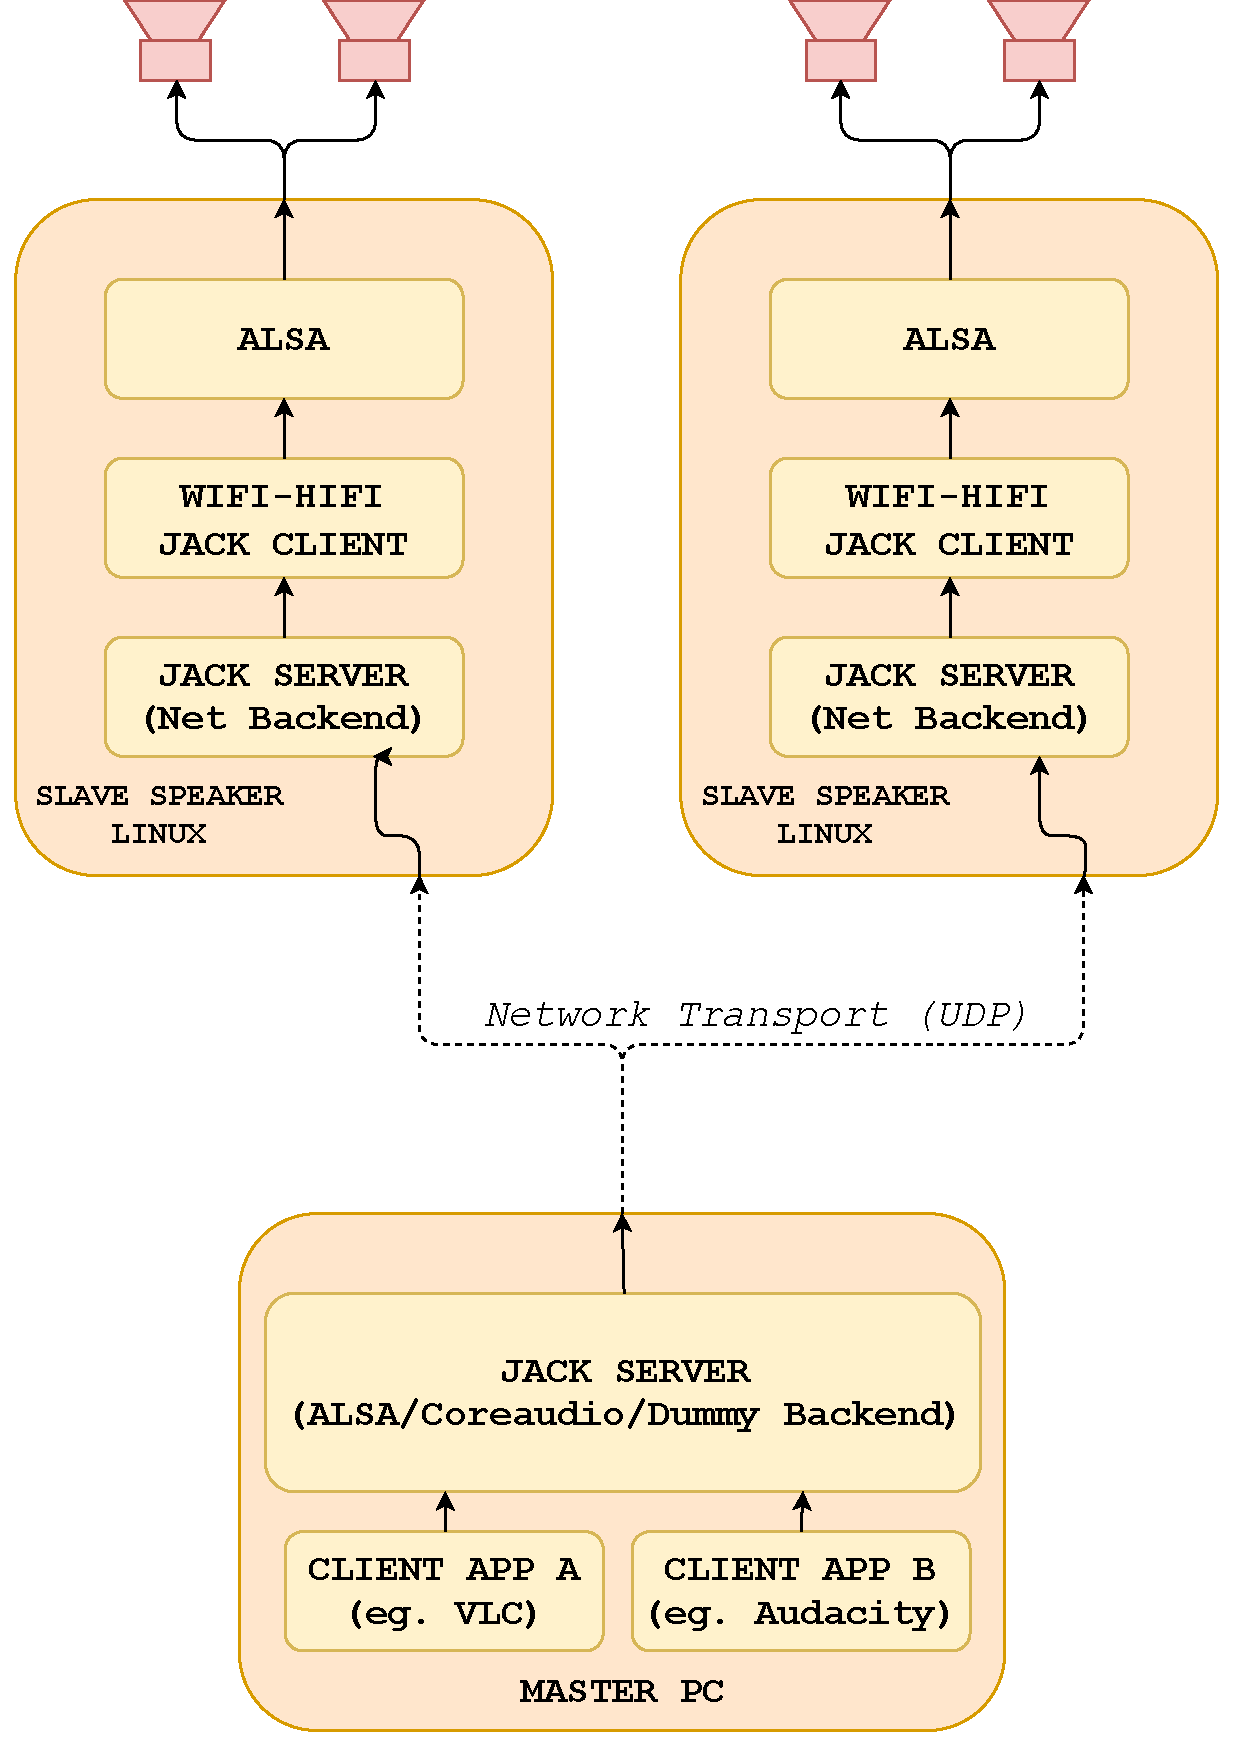
\includegraphics[scale=0.4]{./figs/JACKclients.pdf}
    
    \caption{High-level JACK-based system diagram}
    \label{fig:JACKclients}
\end{figure}

\section{System Startup/Shutdown}

\section{WifiHifi Client}
\subsection{Overview}
%threads, class hierarchy etc
\subsection{Signal Processing}
In order to reduce electronic component count, DSP has been used to implement signal processing tasks that would typically be achieved using analogue circuitry.
These include the crossover filters, frequency correction circuitry and tone controls.
\subsubsection{Crossover Filters}
A two-way crossover circuit is typically used to split the high and low frequencies between the tweeter and woofer respectively around a common crossover frequency using highpass and lowpass filters;
the specific value of this crossover frequency is chosen based on the frequency response of each driver.
As can be seen in figure \ref{fig:tweeter-response}, the resonant frequencies of the tweeter is approximately 1.5kHz.
The crossover frequency was initially set at 3kHz, an octave above the tweeter's resonant frequency.
After some trial and error, it was decided that a crossover frequency of 2.5kHz resulted in the most pleasant response, this is obviously subjective however implementing the filters in software allows them to be varied easily.

\begin{figure}[H]
    \centering
    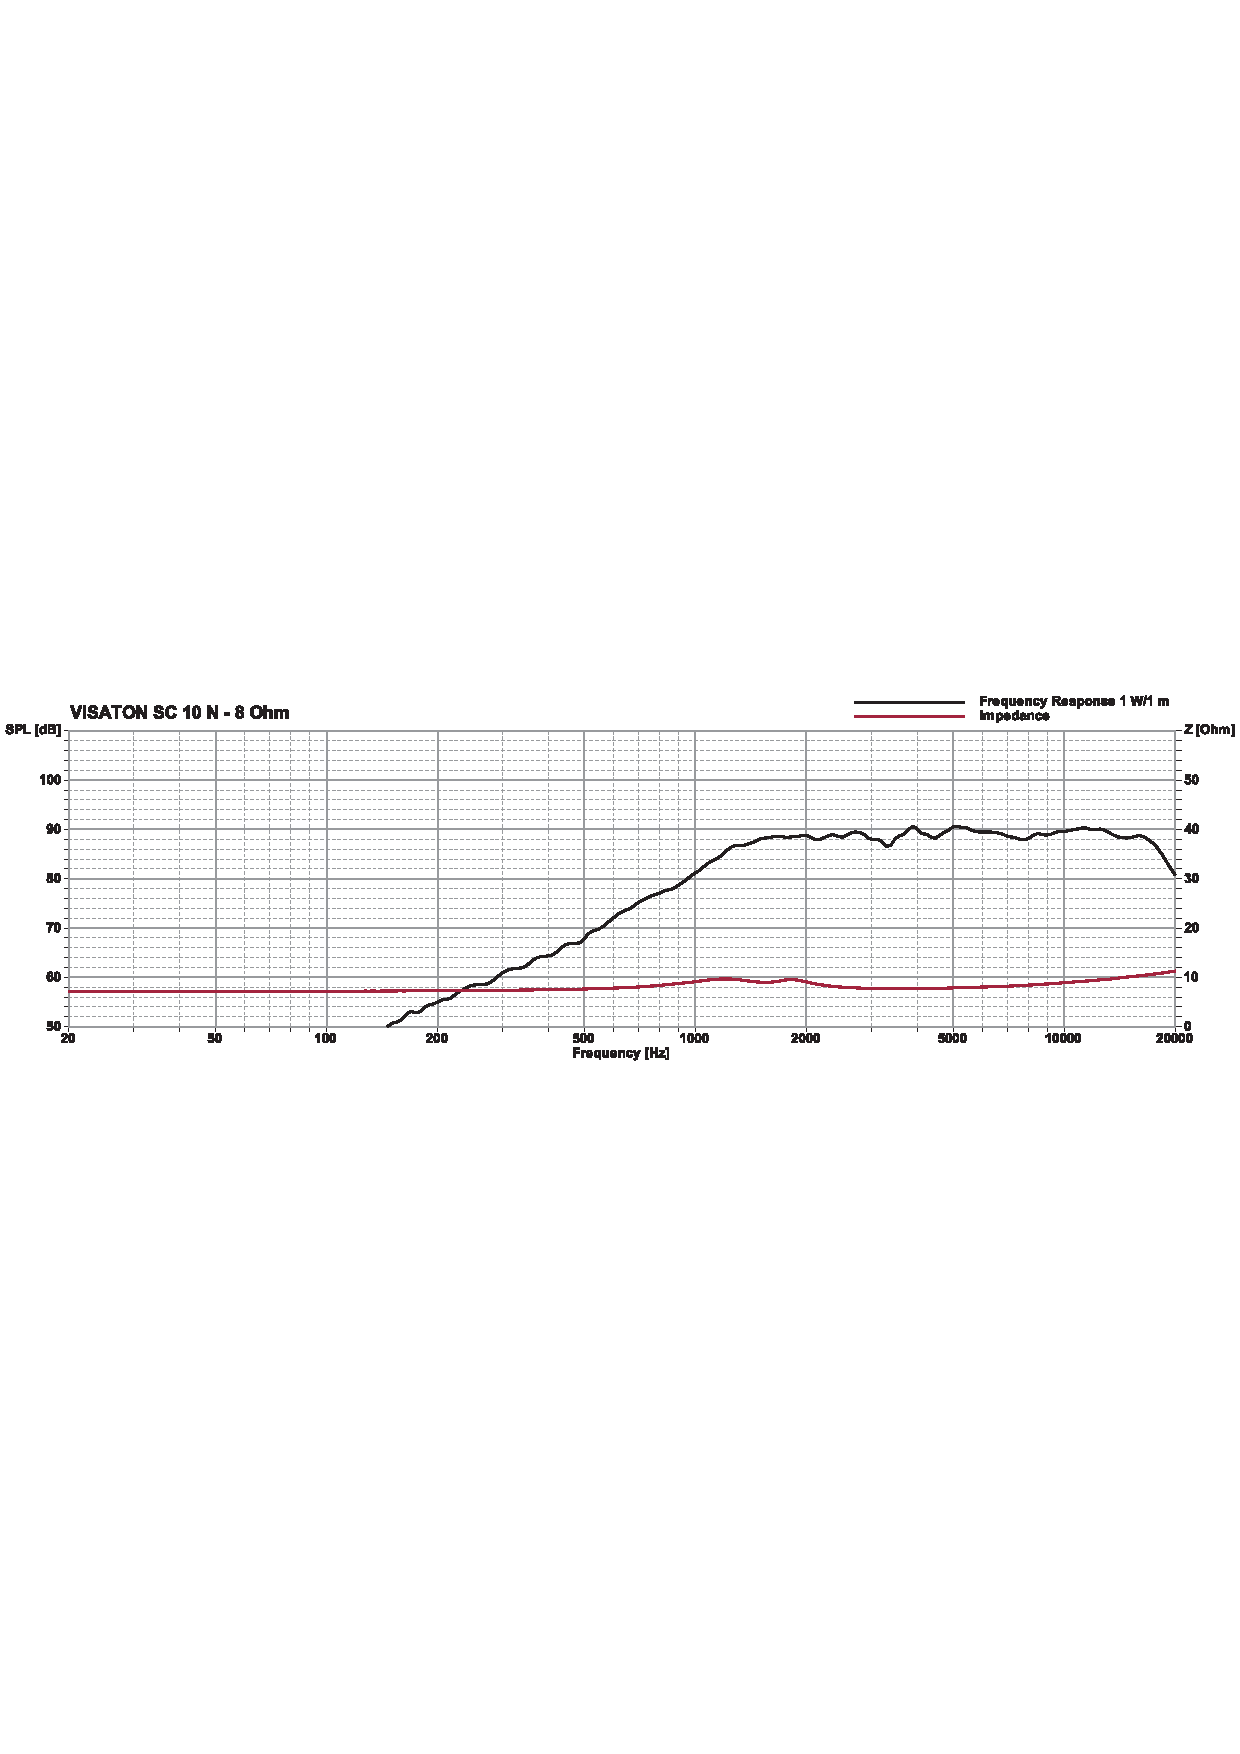
\includegraphics[scale=0.6]{./figs/tweeter-response.pdf}        
    \caption{Impedance and Amplitude response of Tweeter with respect to Frequency\cite{tweeter}}
    \label{fig:tweeter-response}
\end{figure}

\begin{figure}[H]
    \centering
    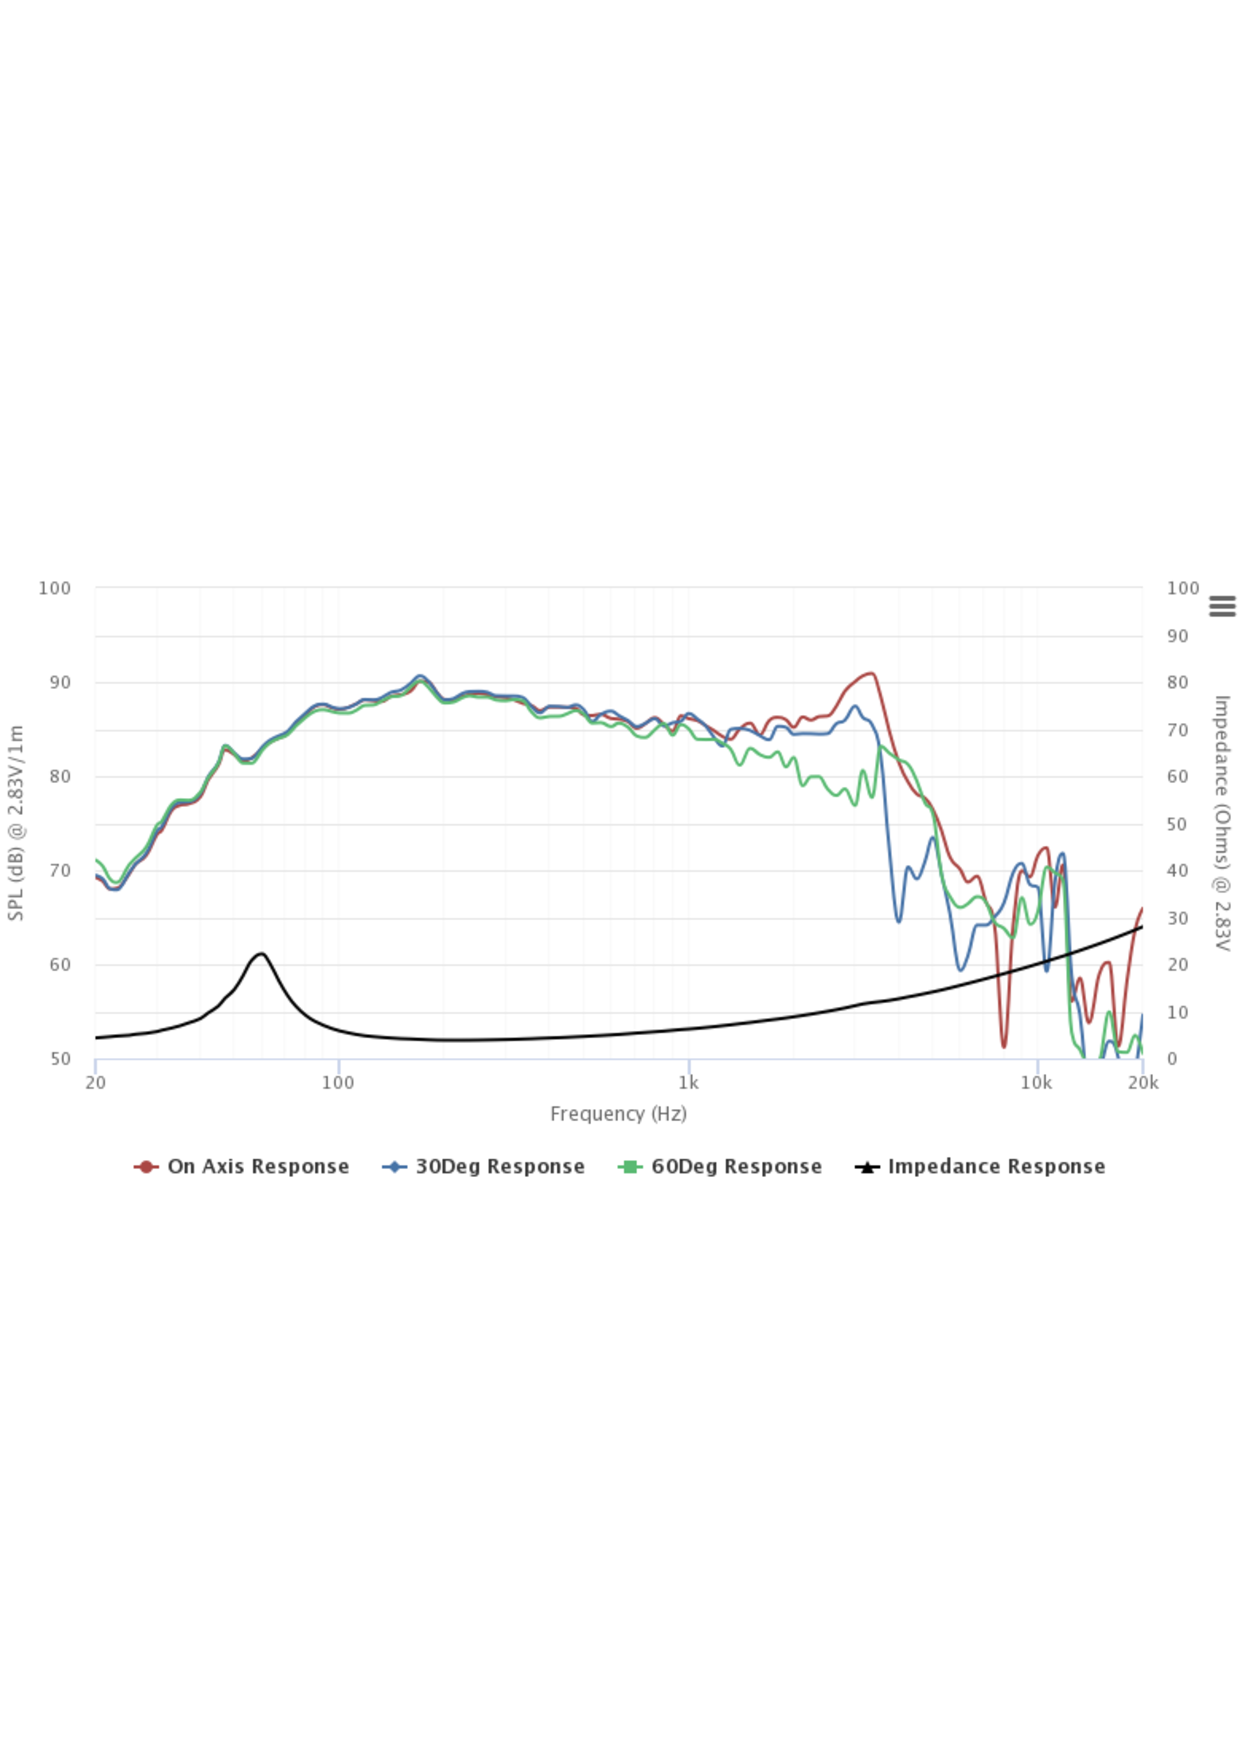
\includegraphics[scale=0.5]{./figs/woofer-response.pdf}        
    \caption{Impedance and Amplitude response of Woofer with respect to Frequency\cite{woofer}}
    \label{fig:woofer-response}
\end{figure}

Each crossover filter was implemented using an FIR filter with 75 coefficients. 
A class (\lstinline{FIRFilter}) was written that calculates the coefficients and performs sample by sample filtering of an input audio sample. 
The filter implementation utilises a real-time FIR filter library written by Bernd Porr\cite{fir1} (\lstinline{fir1}), the calculated coefficients are referenced by an instantiated \lstinline{fir1} object that performs the convolution algorithm. 
A UML class diagram of the \lstinline{FIRFilter} class can be seen in figure \ref{fig:fir-uml}.

\begin{figure}[H]
    \centering
    \begin{tikzpicture}
        \umlclass{WifiHifi::FIRFilter}{  
        - Fir1* : fir \\
        - double* : coeffs 
        }{
        <<constructor>> FIRFilter() \\
        <<destructor>> \char`\~ FIRFilter() \\
        + filter(double) : double \\ 
        + reset() : void \\
        - LowpassCoeffs(int, double) : bool \\
        - HighpassCoeffs(int, double) : bool \\
        - AllpassCoeffs(int) : bool
        }

        \umlclass[x=7.5, y=0]{Fir1}{ 
        - unsigned : taps \\
        - double* : buffer \\
        - double* : coefficients 
        }{
        <<constructor>> Fir1() \\
        <<destructor>> \char`\~ Fir1() \\
        + filter(double) : double \\ 
        + reset() : void \\
        + zeroCoeff() : void \\
        }

        \umlunicompo[geometry=-|]{Fir1}{WifiHifi::FIRFilter}
    \end{tikzpicture}
    \caption{FIRFilter UML Class Diagram}
    \label{fig:fir-uml}
\end{figure}

\medskip
On object construction, the class will numerically calculate the filter impulse response for the specified filter type and number of coefficents/taps. 
The impulse responses are calculated using the following equations\cite{DSP-berndporr}, where $h(n)$, $n$ and $\omega _c$ represent the filter impulse response, current sample and angular cutoff frequency ($\omega _c = 2\pi f_c$) respectively.

\begin{equation}
    h_{lowpass}(n) =
    \begin{cases}
        \frac{\omega _c}{\pi}     &\text{for \(n=0\)}  \\
        \frac{1}{\pi n}sin(\omega _cn)    &\text{else}
    \end{cases}
\end{equation}
\begin{equation}
    h_{highpass}(n) =
    \begin{cases}
        1-\frac{\omega _c}{\pi}     &\text{for \(n=0\)}  \\
        -\frac{1}{\pi n}sin(\omega _cn)    &\text{else}
    \end{cases}
\end{equation}

\medskip
The impulse response is then windowed with a Blackman window.
This was chosen due to its greater attenuation in the stop band than a Hamming window\cite{DSP-berndporr}.
It was calculated using the following equation where $w(n)$, $n$ and $M$ are the window function, current sample and number of coefficients/taps respectively.

\begin{equation}
    w(n)=
    0.42 + 0.5cos\left(\frac{2\pi n}{M}\right) + 0.08cos\left(\frac{4\pi n}{M}\right)
\end{equation}

Figures \ref{fig:tweeter-fft} and \ref{fig:woofer-fft} show plots of FFTs recorded for the highpass and lowpass filters respectively.
They were obtained by probing the relevant DAC output line and passing Gaussian white noise through the WifiHifi client, all other software filtering was disabled.

\begin{figure}[H]
    \centering
    \caption{FFT of Highpass Crossover Filter}
    \label{fig:tweeter-fft}
\end{figure}

\begin{figure}[H]
    \centering
    \caption{FFT of Lowpass Crossover Filter}
    \label{fig:woofer-fft}
\end{figure}

\subsubsection{Frequency Correction}
After crossover filtering, each signal for the tweeter and woofer will typically be subjected to signal processing in an attempt to compensate for undesirable effects caused by the characteristics of each driver.
This is traditionally achieved using analogue circuitry; however, in order to reduce component count, an attempt was made to perform this processing using a custom IIR filter class (\lstinline{IIRFilter}).
A UML class diagram for the \lstinline{IIRFilter} can be seen in the following listing .......


\medskip
The class calculates the filter coefficients during object construction for the specified filter type using equations derived using a Butterworth analogue prototype transfer function and digitising it using the Bilinear transform;
an example derivation can be seen by Bristow-Johnson at \cite{biquad-cookbook}.
The filter implementation was written using a Direct Form I biquad topology, two dual sample buffers are used to as delay lines to multiply fed-forward and fed-back samples by the relevant coefficients.
The $a_0$ coefficient is simply used as an attenuation factor for the output accumulator.
A block diagram of the biquad filter can be seen in figure \ref{fig:biquad}
\begin{figure}[H]
    \centering
    \begin{signalflow}{}
        % - delay element
        \begin{scope}
            \node [input] (in) {$x(n)$};
            \node [node] (node1) [right from=in] {};
            \node [multiplier] (b0) [right from=node1] {\nodepart{above}{$b_0$}};
            \node [adder]  (accum) [right from=b0]  {$\Sigma$};
            \node [delay] (del1) [below from=node1, fill=lightgray] {$T$};
            \node [multiplier] (b1) [below from=b0] {\nodepart{above}{$b_1$}};
            \node [delay] (del2) [below from=del1, fill=lightgray] {$T$}; 
            \node [multiplier] (b2) [below from=b1] {\nodepart{above}{$b_2$}};
            \node [adder] (accumFF) [below from=accum] {$\Sigma$};
            \node [adder] (accum2) [right from=accum] {$\Sigma$};
            \node [node] (node0) [right from=accum2, fill=white, draw=white] {};
            \node [node] (node2) [right from=node0] {};
            \node [adder] (accumFB) [below from=accum2] {$\Sigma$};
            \node [multiplier] (a1) [right from=accumFB] {\nodepart{above}{$a_1$}};
            \node [delay] (del3) [below from=node2, fill=lightgray] {$T$}; 
            \node [multiplier] (a2) [below from=a1] {\nodepart{above}{$a_2$}};
            \node [delay] (del4) [below from=del3, fill=lightgray] {$T$};    
            \node [output] (out) [right from=node2] {$y(n)$};

            % signal paths
            \path[r] (in)  -- (node1);
            \path[r>] (node1)  -- (b0);
            \path[r>] (b0)  -- (accum);
            \path[r>] (node1) -- (del1);
            \path[r>] (del1) -- (del2);
            \path[r>] (del1) -- (b1);
            \path[r>] (b1) -- (accumFF);
            \path[r>] (del2) -- (b2);
            \path[r>] (b2) -| (accumFF);
            \path[r>] (accumFF) -- (accum);
            \path[r>] (accum) -- (accum2);
            \path[r>] (node2) -- (del3);
            \path[r>] (del3) -- (del4);
            \path[r>] (del3) -- (a1);
            \path[r>] (del4) -- (a2);
            \path[r>] (a1) -- (accumFB);
            \path[r>] (a2) -| (accumFB);
            \path[r>] (accumFB) -- (accum2);            
            \path[r] (accum2) -- (node2);
            \path[r>] (node2) -- (out);
        \end{scope}
    \end{signalflow}
    \caption{Direct Form I Biquad IIR Filter}
    \label{fig:biquad}
\end{figure}

\medskip
A notch filter is normally implemented on the high frequency signal to counteract the tweeters resonant frequency, this is traditionally done using either an active or passive bandstop circuit.
An instantiated \lstinline{IIRFilter} object configured as a bandstop filter is used as an alternative to an analogue solution, the filter coefficients are calculated during construction using the following equations.

\begin{center}
\noindent\begin{minipage}{.3\linewidth}
    \begin{equation*}
        \begin{aligned} 
            &a_0 = 1 + \alpha \\
            &a_1 = -2cos(\omega _0) \\
            &a_2 = 1 - \alpha
        \end{aligned}
    \end{equation*}
    \end{minipage}%
    \begin{minipage}{.3\linewidth}
    \begin{equation*}
        \begin{aligned}
            &b_0 = 1 \\
            &b_1 = -2cos(\omega _0) \\
            &b_2 = 1 
        \end{aligned}
    \end{equation*}
\end{minipage}
\end{center}

\medskip
A zobel network, a series resistor and capacitor, is normally placed in parallel with the woofer to counteract the impedance rise at higher frequencies caused by the driver's voice-coil inductance. 
In an effort to reduce the rising frequency towards the crossover, a high shelve \lstinline{IIRFilter} object with an attenuation of -12dB was used, the filter coefficients are calculated during construction using the following equations, 
where $A = \sqrt{10^{\frac{dBgain}{20}}}$ .

\begin{center}
    \begin{minipage}{.5\linewidth}
        \begin{equation*}
            \begin{aligned} 
                &a_0 = (A + 1) - (A - 1)cos(\omega_ 0) + 2\sqrt{A} \alpha \\
                &a_1 = 2((A - 1) - (A + 1)cos(\omega_ 0)) \\
                &a_2 = (A + 1) - (A - 1)cos(\omega_ 0) - 2\sqrt{A} \alpha
            \end{aligned}
        \end{equation*}
        \end{minipage}%
        \begin{minipage}{.5\linewidth}
        \begin{equation*}
            \begin{aligned}
                &b_0 = A((A + 1) + (A - 1)cos(\omega _0) + 2\sqrt{A} \alpha) \\
                &b_1 = -2A((A - 1) + (A + 1)cos(\omega _0)) \\
                &b_2 = A((A + 1) + (A - 1)cos(\omega_ 0) - 2\sqrt{A} \alpha)
            \end{aligned}
        \end{equation*}
    \end{minipage}
    \end{center}

\medskip 


\subsubsection{3-Band EQ}
\subsubsection{Results}
\subsection{ALSA Interface}
% interleaving etc
\subsection{User I/O}

\section{Drift Correction}
\subsection{Overview}
%describe algorithm/maths
\subsection{Implementation}
\subsection{Results}
\begin{tikzpicture}
    \begin{axis}[
        width=\textwidth, 
        height=\axisdefaultheight, 
        xtick={0,1,...,10},
        xmin=0,
        xmax=10]
    %\addplot table [mark=none, x=t, y=a, col sep=comma] {./data/saleae-outputs/sync.csv};
    
    \addplot table [mark=none, x=t, y=b, col sep=comma] {./data/saleae-outputs/run1.csv};
    \end{axis}
\end{tikzpicture}

\section{Desktop Application}
\subsection{Overview}
\subsection{Tone Controls}
\subsection{Connection Protocol}

\end{document}